\documentclass[11pt,a4paper]{report}
\usepackage[textwidth=37em,vmargin=30mm]{geometry}
\usepackage{calc,xunicode,amsmath,amssymb,paralist,enumitem,tabu,booktabs,datetime2,xeCJK,xeCJKfntef,listings}
\usepackage{tocloft,fancyhdr,tcolorbox,xcolor,graphicx,eso-pic,xltxtra,xelatexemoji}

\newcommand{\envyear}[0]{2024}
\newcommand{\envdatestr}[0]{2024-10-24}
\newcommand{\envfinaldir}[0]{webdb/2024/20241024/final}

\usepackage[hidelinks]{hyperref}
\hypersetup{
    colorlinks=false,
    pdfpagemode=FullScreen,
    pdftitle={Web Digest - \envdatestr}
}

\setlength{\cftbeforechapskip}{10pt}
\renewcommand{\cftchapfont}{\rmfamily\bfseries\large\raggedright}
\setlength{\cftbeforesecskip}{2pt}
\renewcommand{\cftsecfont}{\sffamily\small\raggedright}

\setdefaultleftmargin{2em}{2em}{1em}{1em}{1em}{1em}

\usepackage{xeCJK,xeCJKfntef}
\xeCJKsetup{PunctStyle=plain,RubberPunctSkip=false,CJKglue=\strut\hskip 0pt plus 0.1em minus 0.05em,CJKecglue=\strut\hskip 0.22em plus 0.2em}
\XeTeXlinebreaklocale "zh"
\XeTeXlinebreakskip = 0pt


\setmainfont{Brygada 1918}
\setromanfont{Brygada 1918}
\setsansfont{IBM Plex Sans}
\setmonofont{JetBrains Mono NL}
\setCJKmainfont{Noto Serif CJK SC}
\setCJKromanfont{Noto Serif CJK SC}
\setCJKsansfont{Noto Sans CJK SC}
\setCJKmonofont{Noto Sans CJK SC}

\setlength{\parindent}{0pt}
\setlength{\parskip}{8pt}
\linespread{1.15}

\lstset{
	basicstyle=\ttfamily\footnotesize,
	numbersep=5pt,
	backgroundcolor=\color{black!5},
	showspaces=false,
	showstringspaces=false,
	showtabs=false,
	tabsize=2,
	captionpos=b,
	breaklines=true,
	breakatwhitespace=true,
	breakautoindent=true,
	linewidth=\textwidth
}






\newcommand{\coverpic}[2]{
    % argv: itemurl, authorname
    Cover photo by #2~~(\href{#1}{#1})
}
\newcommand{\makeheader}[0]{
    \begin{titlepage}
        % \newgeometry{hmargin=15mm,tmargin=21mm,bmargin=12mm}
        \begin{center}
            
            \rmfamily\scshape
            \fontspec{BaskervilleF}
            \fontspec{Old Standard}
            \fontsize{59pt}{70pt}\selectfont
            WEB\hfill DIGEST
            
            \vfill
            % \vskip 30pt
            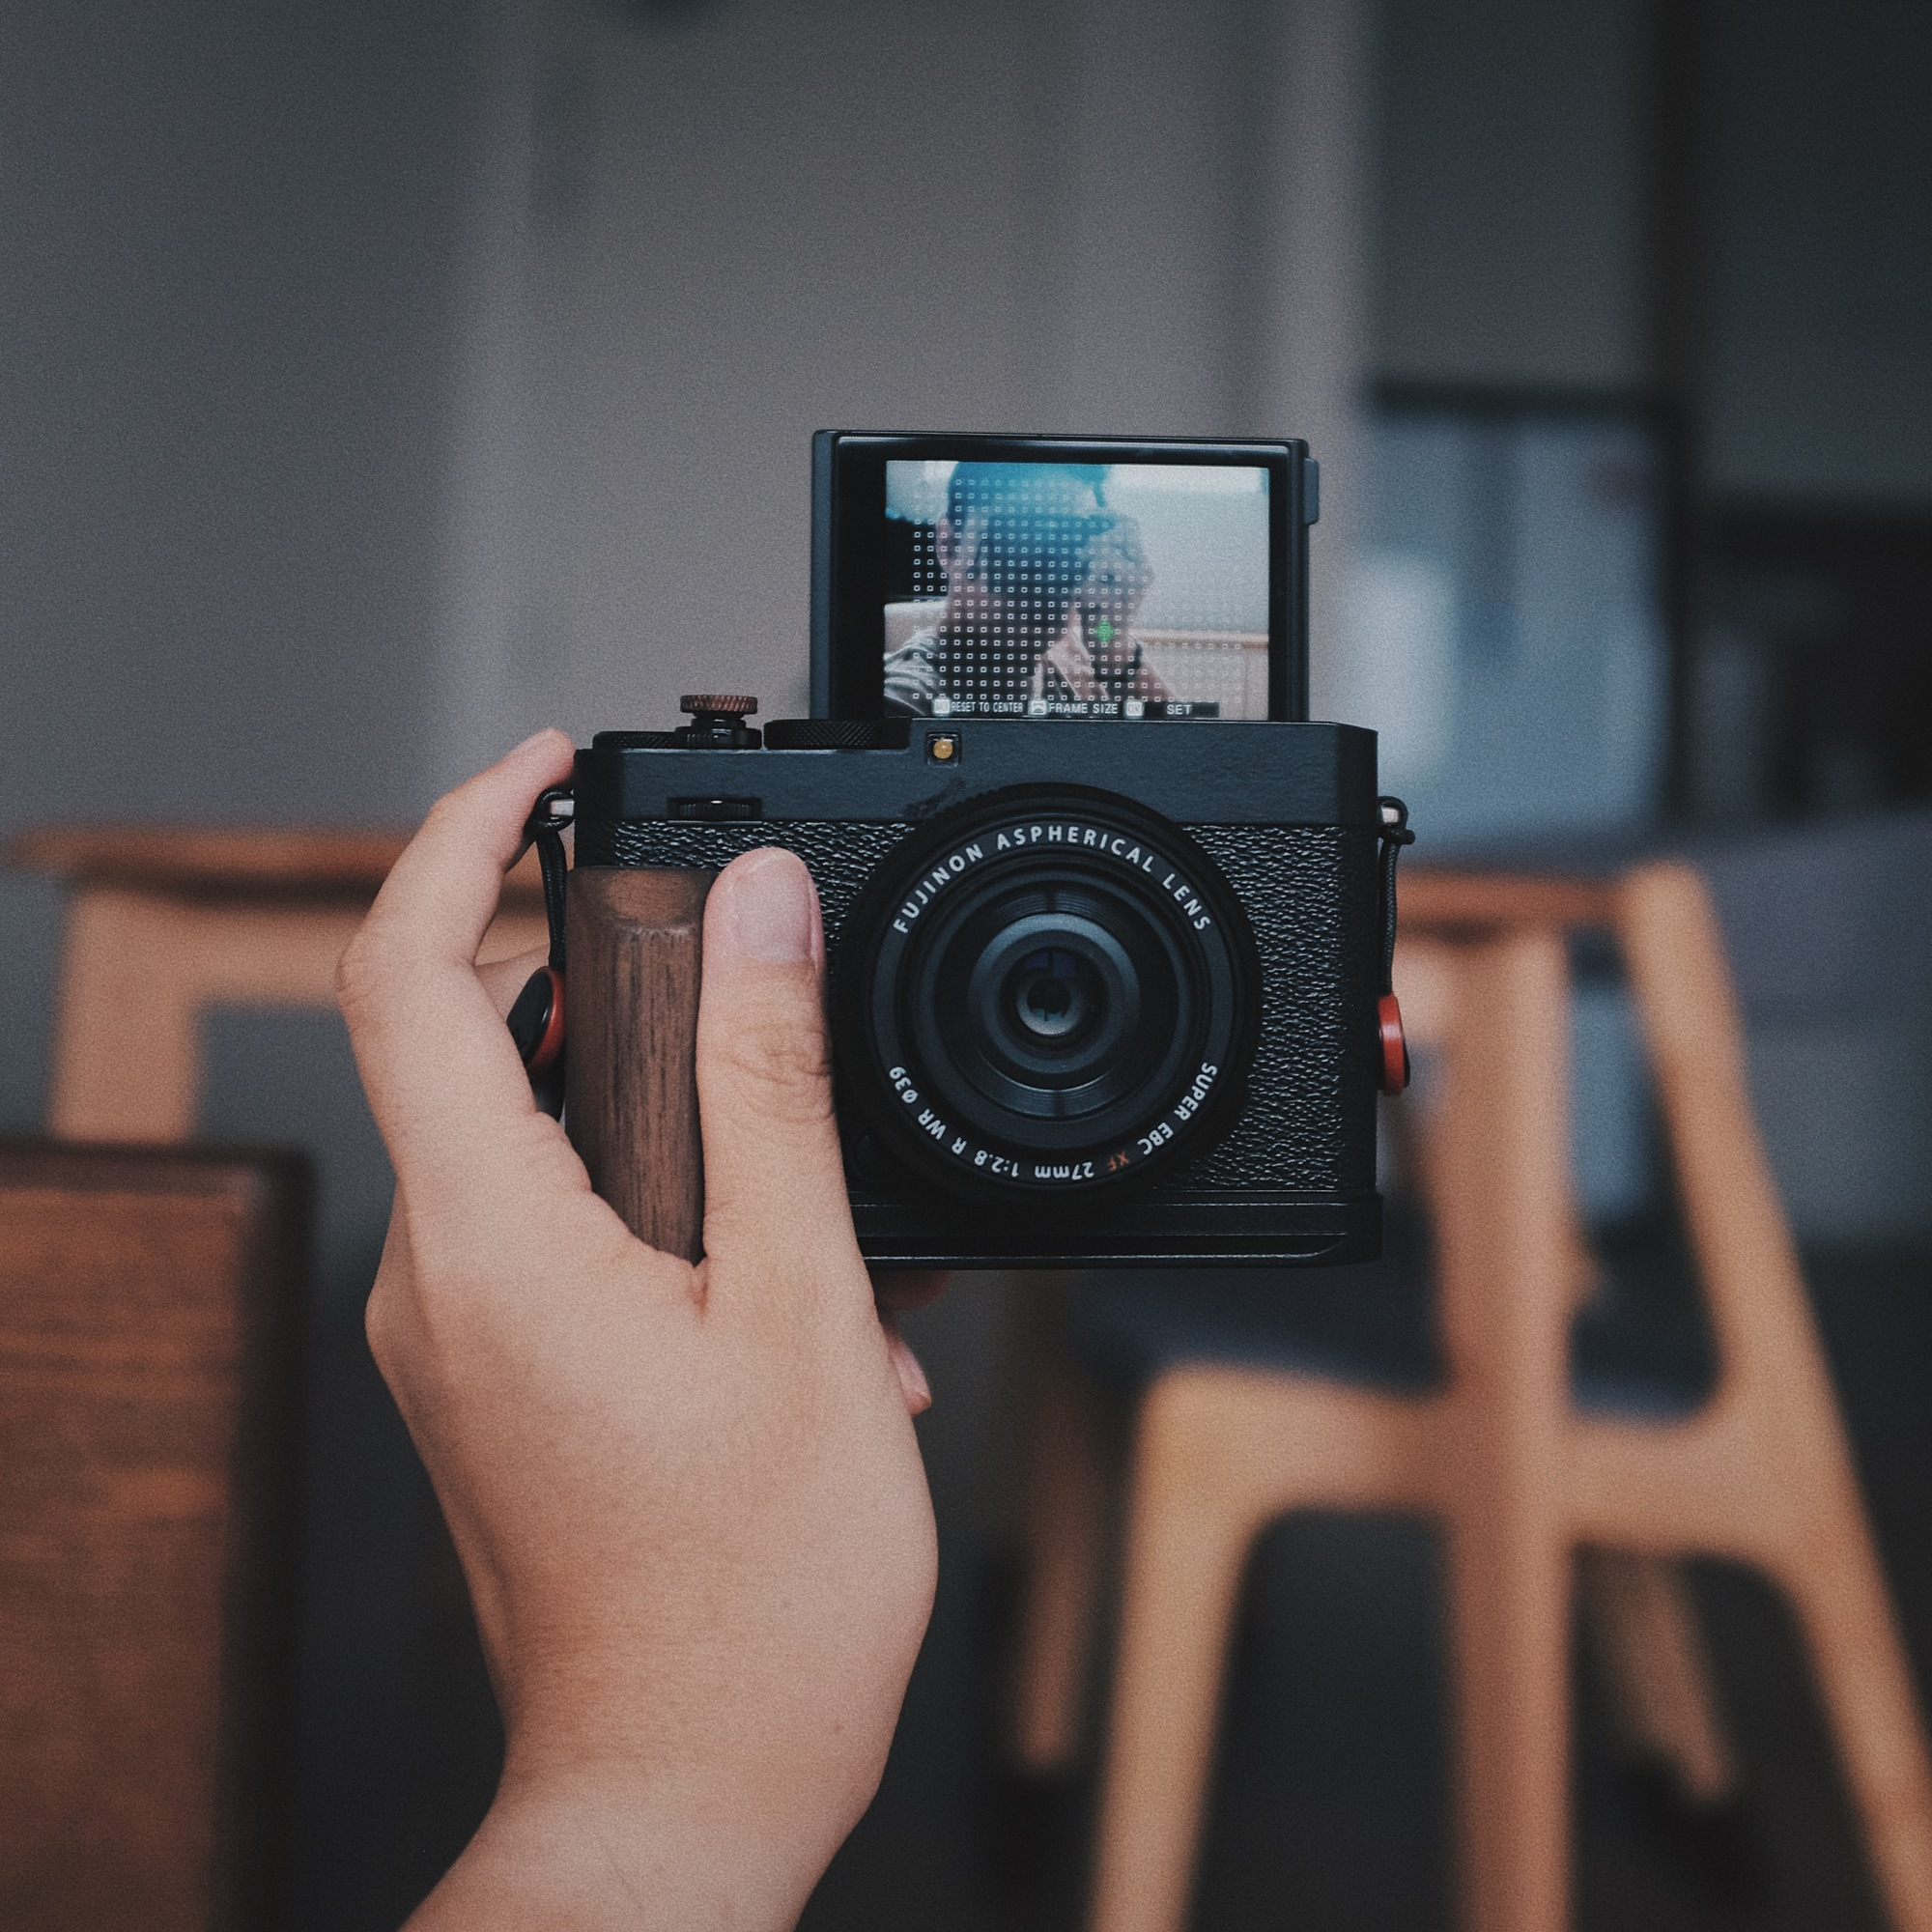
\includegraphics[width=\linewidth]{\envfinaldir/coverpic-prod.jpg}\par
            % \vskip 30pt
            \vfill

            \normalsize\rmfamily\scshape
            \copyright{} The Web Digest Project \hfill\large \envdatestr
        \end{center}
    \end{titlepage}
    % \restoregeometry
}
\newcommand{\simplehref}[1]{%
    \textcolor{blue!80!green}{\href{#1}{#1}}%
}
\renewcommand{\contentsname}{\center\Huge\sffamily\bfseries Contents\par\vskip 20pt}
\newcounter{ipartcounter}
\setcounter{ipartcounter}{0}
\newcommand{\ipart}[1]{
    % \vskip 20pt
    \clearpage
    \stepcounter{ipartcounter}
    \phantomsection
    \addcontentsline{toc}{chapter}{#1}
    % \begin{center}
    %     \Huge
    %     \sffamily\bfseries
    %     #1
    % \end{center}
    % \vskip 20pt plus 7pt
}
\newcounter{ichaptercounter}
\setcounter{ichaptercounter}{0}
\newcommand{\ichapter}[1]{
    % \vskip 20pt
    \clearpage
    \stepcounter{ichaptercounter}
    \phantomsection
    \addcontentsline{toc}{section}{\numberline{\arabic{ichaptercounter}}#1}
    \begin{center}
        \Huge
        \sffamily\bfseries
        #1
    \end{center}
    \vskip 20pt plus 7pt
}
\newcommand{\entrytitlefont}[1]{\subsection*{\raggedright\Large\sffamily\bfseries#1}}
\newcommand{\entryitemGeneric}[2]{
    % argv: title, url
    \parbox{\linewidth}{
        \entrytitlefont{#1}\par\vskip 5pt
        \footnotesize\ttfamily\mdseries
        \simplehref{#2}
    }\vskip 11pt plus 11pt minus 1pt
}
\newcommand{\entryitemGithub}[3]{
    % argv: title, url, desc
    \parbox{\linewidth}{
        \entrytitlefont{#1}\par\vskip 5pt
        \footnotesize\ttfamily\mdseries
        \simplehref{#2}\par\vskip 5pt
        \small\rmfamily\mdseries#3
    }\vskip 11pt plus 11pt minus 1pt
}
\newcommand{\entryitemAp}[3]{
    % argv: title, url, desc
    \parbox{\linewidth}{
        \entrytitlefont{#1}\par\vskip 5pt
        \footnotesize\ttfamily\mdseries
        \simplehref{#2}\par\vskip 5pt
        \small\rmfamily\mdseries#3
    }\vskip 11pt plus 11pt minus 1pt
}
\newcommand{\entryitemHackernews}[3]{
    % argv: title, hnurl, rawurl
    % \parbox{\linewidth}{
    %     \entrytitlefont{#1}\par\vskip 5pt
    %     \footnotesize\ttfamily\mdseries
    %     \simplehref{#3}\par
    %     \textcolor{black!50}{\href{#2}{#2}}
    % }\vskip 11pt plus 11pt minus 1pt
    \begin{minipage}{\linewidth}
            \entrytitlefont{#1}\par\vskip 5pt
            \footnotesize\ttfamily\mdseries
            \simplehref{#3}\par
            \textcolor{black!50}{\href{#2}{#2}}
    \end{minipage}\par\vskip 11pt plus 11pt minus 1pt
}







\begin{document}

\makeheader

\tableofcontents\clearpage




\ipart{Developers}
\ichapter{Hacker News}
\entryitemTwoLinks{Everything I built with Claude Artifacts this week}{https://news.ycombinator.com/item?id=41929174}{https://simonwillison.net/2024/Oct/21/claude-artifacts/}

\entryitemTwoLinks{Playstation Vita Architecture (Part 1)}{https://news.ycombinator.com/item?id=41928529}{https://www.copetti.org/writings/consoles/playstation-vita/}

\entryitemTwoLinks{Goldman and Apple 'illegally sidestepped' obligations to credit-card customers}{https://news.ycombinator.com/item?id=41926978}{https://finance.yahoo.com/news/goldman-and-apple-illegally-sidestepped-obligations-to-credit-card-customers-cfpb-161226158.html}

\entryitemTwoLinks{Show HN: Agent.exe, a cross-platform app to let 3.5 Sonnet control your machine}{https://news.ycombinator.com/item?id=41926770}{https://github.com/corbt/agent.exe}

\entryitemTwoLinks{Paper mills: the 'cartel-like' companies behind fraudulent scientific journals}{https://news.ycombinator.com/item?id=41926515}{https://theconversation.com/paper-mills-the-cartel-like-companies-behind-fraudulent-scientific-journals-230124}

\entryitemTwoLinks{Lawsuit challenges Virginia City's use of cameras for warrantless surveillance}{https://news.ycombinator.com/item?id=41926472}{https://ij.org/press-release/federal-lawsuit-challenges-virginia-citys-use-of-over-170-cameras-to-conduct-prolonged-warrantless-surveillance-of-entire-driving-population/}

\entryitemTwoLinks{RISC-V is currently slow compared to modern CPUs}{https://news.ycombinator.com/item?id=41925511}{https://benhouston3d.com/blog/risc-v-in-2024-is-slow}

\entryitemTwoLinks{The global surveillance free-for-all in mobile ad data}{https://news.ycombinator.com/item?id=41923931}{https://krebsonsecurity.com/2024/10/the-global-surveillance-free-for-all-in-mobile-ad-data/}

\entryitemTwoLinks{Probably pay attention to tokenizers}{https://news.ycombinator.com/item?id=41923625}{https://cybernetist.com/2024/10/21/you-should-probably-pay-attention-to-tokenizers/}

\entryitemTwoLinks{Huawei makes divorce from Android official with HarmonyOS NEXT launch}{https://news.ycombinator.com/item?id=41923387}{https://www.theregister.com/2024/10/23/huaweis\_harmonyos\_next\_launch/}

\entryitemTwoLinks{What happens when you make a move in lichess.org?}{https://news.ycombinator.com/item?id=41922928}{https://www.davidreis.me/2024/what-happens-when-you-make-a-move-in-lichess}

\entryitemTwoLinks{Adding row polymorphism to Damas-Hindley-Milner}{https://news.ycombinator.com/item?id=41922081}{https://bernsteinbear.com/blog/row-poly/}

\entryitemTwoLinks{One Square Minesweeper}{https://news.ycombinator.com/item?id=41921703}{https://onesquareminesweeper.com/}

\entryitemTwoLinks{Arm is canceling Qualcomm's chip design license}{https://news.ycombinator.com/item?id=41920401}{https://www.bloomberg.com/news/articles/2024-10-23/arm-to-cancel-qualcomm-chip-design-license-in-escalation-of-feud}

\entryitemTwoLinks{The Forest Service Is Losing 2,400 Jobs–Including Most of Its Trail Workers}{https://news.ycombinator.com/item?id=41920127}{https://www.backpacker.com/news-and-events/news/us-forest-service-job-eliminations-trail-workers/}

\entryitemTwoLinks{A new book shows how the power of companies is destabilizing governance}{https://news.ycombinator.com/item?id=41919907}{https://hai.stanford.edu/news/tech-coup-new-book-shows-how-unchecked-power-companies-destabilizing-governance}

\entryitemTwoLinks{Simone Giertz talks about invention}{https://news.ycombinator.com/item?id=41919717}{https://spectrum.ieee.org/simone-giertz}

\entryitemTwoLinks{The Dawn of a New Era for Supernova 1987a (2017)}{https://news.ycombinator.com/item?id=41919711}{https://science.nasa.gov/missions/chandra/the-dawn-of-a-new-era-for-supernova-1987a/}

\entryitemTwoLinks{Several Russian developers lose kernel maintainership status}{https://news.ycombinator.com/item?id=41919670}{https://lwn.net/Articles/995186/}

\entryitemTwoLinks{I got dysentery so you don't have to}{https://news.ycombinator.com/item?id=41919365}{https://eukaryotewritesblog.com/2024/10/21/i-got-dysentery-so-you-dont-have-to/}\ichapter{Phoronix}
\entryitemGeneric{\hskip 0pt{}Intel Core Ultra 7 "Lunar Lake" Performance Up By ~22\% With ASUS Linux Fix}{https://www.phoronix.com/review/lunar-lake-linux-improved}

\entryitemGeneric{\hskip 0pt{}Linus Torvalds Comments On The Russian Linux Maintainers Being Delisted}{https://www.phoronix.com/news/Linus-Torvalds-Russian-Devs}

\entryitemGeneric{\hskip 0pt{}Gentoo Linux Touts DTrace 2.0 Support}{https://www.phoronix.com/news/Gentoo-Linux-DTrace-2.0}

\entryitemGeneric{\hskip 0pt{}Significant CRC32C Throughput Optimization On The Way To The Linux Kernel}{https://www.phoronix.com/news/Linux-Faster-CRC32X-x86}

\entryitemGeneric{\hskip 0pt{}Intel Preps PXP GuC Auto-Teardown \& Improvements For Old iGPUs With Linux 6.13}{https://www.phoronix.com/news/Intel-PXP-GuC-Auto-Teardown}

\entryitemGeneric{\hskip 0pt{}Linux 6.13 To Default To AMD P-State Driver For EPYC 9005 CPUs}{https://www.phoronix.com/news/AMD-P-State-EPYC-Linux-6.13}

\entryitemGeneric{\hskip 0pt{}Cloudflare Continues To Praise Open-Source OpenBMC}{https://www.phoronix.com/news/Cloudflare-OpenBMC-2024}

\entryitemGeneric{\hskip 0pt{}The Free Software Foundation Finally Has AI / Machine Learning Apps On Their Radar}{https://www.phoronix.com/news/FSF-Freedom-AI-ML-Software}

\entryitemGeneric{\hskip 0pt{}Rust-Written Rustls Now Reportedly Outperforming OpenSSL \& BoringSSL}{https://www.phoronix.com/news/Rustls-Faster-Than-OpenSSL}


\ipart{Developers~~~~(zh-Hans)}
\ichapter{Solidot}
\entryitemGeneric{\hskip 0pt{}维基百科遵守印度法庭命令删除了一个条目}{https://www.solidot.org/story?sid=79570}

\entryitemGeneric{\hskip 0pt{}日本公布了其候选登月宇航员}{https://www.solidot.org/story?sid=79569}

\entryitemGeneric{\hskip 0pt{}数学家仍然在追赶拉马努金的神来之手}{https://www.solidot.org/story?sid=79568}

\entryitemGeneric{\hskip 0pt{}Arm 向高通发出取消芯片设计授权的通知}{https://www.solidot.org/story?sid=79567}

\entryitemGeneric{\hskip 0pt{}30 亿年前撞击地球的陨石让海洋为之沸腾}{https://www.solidot.org/story?sid=79566}

\entryitemGeneric{\hskip 0pt{}亚马逊声称其反工会策略受到宪法第一修正案的保护}{https://www.solidot.org/story?sid=79565}

\entryitemGeneric{\hskip 0pt{}Meta 封禁了跟踪扎克伯格和马斯克私人飞机的账号}{https://www.solidot.org/story?sid=79564}

\entryitemGeneric{\hskip 0pt{}Linux 项目以合规为由移除了多名俄籍维护者}{https://www.solidot.org/story?sid=79562}

\entryitemGeneric{\hskip 0pt{}波音和英特尔的危机被认为危及美国国家安全}{https://www.solidot.org/story?sid=79561}

\entryitemGeneric{\hskip 0pt{}苹果更新 iOS 计算器移除 C 按键}{https://www.solidot.org/story?sid=79560}

\entryitemGeneric{\hskip 0pt{}Google Scholar 认证了牛顿爵士的电邮}{https://www.solidot.org/story?sid=79559}

\entryitemGeneric{\hskip 0pt{}李彦宏预测 AI 是另一个泡沫,99\% 的 AI 公司会在泡沫破裂时面临倒闭}{https://www.solidot.org/story?sid=79558}

\entryitemGeneric{\hskip 0pt{}《Squadron 42》将于 2026 年发布}{https://www.solidot.org/story?sid=79557}

\entryitemGeneric{\hskip 0pt{}被裁的 IT 员工变成前雇主的 IT 外包}{https://www.solidot.org/story?sid=79556}

\entryitemGeneric{\hskip 0pt{}前英伟达工程师发现第 52 个梅森素数}{https://www.solidot.org/story?sid=79555}

\entryitemGeneric{\hskip 0pt{}微软屏蔽两款华硕笔记本更新 Windows 11 24H2}{https://www.solidot.org/story?sid=79554}

\entryitemGeneric{\hskip 0pt{}AI 关键词更可能增加论文引用率}{https://www.solidot.org/story?sid=79553}

\entryitemGeneric{\hskip 0pt{}埃及消灭了疟疾}{https://www.solidot.org/story?sid=79552}

\entryitemGeneric{\hskip 0pt{}政治自恋助长了将政治对手非人化的倾向}{https://www.solidot.org/story?sid=79551}

\entryitemGeneric{\hskip 0pt{}大黄蜂蜂后选择在农药污染的土壤下冬眠}{https://www.solidot.org/story?sid=79550}\ichapter{V2EX}
\entryitemGeneric{\hskip 0pt{}[Google] pixel 7 root 和安装面具之后,有办法无损升级么?}{https://www.v2ex.com/t/1083072}

\entryitemGeneric{\hskip 0pt{}[NAS] 退坑出惠普 hp ProLiant MicroServer gen8 服务器}{https://www.v2ex.com/t/1083071}

\entryitemGeneric{\hskip 0pt{}[Apple] 苹果推送 iOS 18.2 开发者测试版,上线 Genmoji、Image Playground 及 ChatGPT 集成}{https://www.v2ex.com/t/1083070}

\entryitemGeneric{\hskip 0pt{}[iPhone] iOS 18.2 Beta 来了,包含图片生成、Genmoji 和 ChatGPT 集成}{https://www.v2ex.com/t/1083068}

\entryitemGeneric{\hskip 0pt{}[推广] 一个免费的在线裁剪图片工具 - 支持矩形、圆形、心形}{https://www.v2ex.com/t/1083067}

\entryitemGeneric{\hskip 0pt{}[问与答] 付费咨询}{https://www.v2ex.com/t/1083066}

\entryitemGeneric{\hskip 0pt{}[北京] 想看看有没有家长需要家教的}{https://www.v2ex.com/t/1083065}

\entryitemGeneric{\hskip 0pt{}[分享发现] follow 开启公厕}{https://www.v2ex.com/t/1083064}

\entryitemGeneric{\hskip 0pt{}[程序员] 今天是 1024。}{https://www.v2ex.com/t/1083063}

\entryitemGeneric{\hskip 0pt{}[宽带症候群] 找一个办宽带的营业员,四川德阳地区}{https://www.v2ex.com/t/1083062}

\entryitemGeneric{\hskip 0pt{}[摄影] 想买一个运动相机作为定点录像的副机位,有没有推荐}{https://www.v2ex.com/t/1083061}

\entryitemGeneric{\hskip 0pt{}[分享创造] 做了一个 AI 图片站,最近比较热的 Stable Diffusion 3.5}{https://www.v2ex.com/t/1083060}

\entryitemGeneric{\hskip 0pt{}[投资] 这两天的投资笔记}{https://www.v2ex.com/t/1083058}

\entryitemGeneric{\hskip 0pt{}[Android] android 应用是不是自动添加开机启动权限?}{https://www.v2ex.com/t/1083057}

\entryitemGeneric{\hskip 0pt{}[问与答] 容器中的 nginx 正确反代其它容器的姿势是什么?}{https://www.v2ex.com/t/1083056}

\entryitemGeneric{\hskip 0pt{}[Android] emby 安卓版播放 hdr 电影是不是有问题?}{https://www.v2ex.com/t/1083055}

\entryitemGeneric{\hskip 0pt{}[问与答] 兄弟们有没有 oracle 的奇淫巧技推荐下}{https://www.v2ex.com/t/1083054}

\entryitemGeneric{\hskip 0pt{}[YouTube] 美国家庭组 YOUTUBE PREMIUM 拼车, 老车差 1 个人}{https://www.v2ex.com/t/1083053}

\entryitemGeneric{\hskip 0pt{}[职场话题] 回旋的 86}{https://www.v2ex.com/t/1083052}

\entryitemGeneric{\hskip 0pt{}[Android] 有老哥逆向分析过小米解锁 bl 的 mi unlock 吗?}{https://www.v2ex.com/t/1083051}

\entryitemGeneric{\hskip 0pt{}[汽车] 车 or 房 or 存}{https://www.v2ex.com/t/1083050}

\entryitemGeneric{\hskip 0pt{}[Apple] 新的 mini AC 的价格为啥是 2 年 ¥299?}{https://www.v2ex.com/t/1083049}

\entryitemGeneric{\hskip 0pt{}[问与答] 如何在不进行实名认证及不绑定支付方式的前提下,在 Upwork 平台发布招聘信息?}{https://www.v2ex.com/t/1083048}

\entryitemGeneric{\hskip 0pt{}[游戏] 推荐个高质量的网站,有几百款在线游戏}{https://www.v2ex.com/t/1083047}

\entryitemGeneric{\hskip 0pt{}[Android] 小米 12spro 老哥们有没有被施法 作为弃舰机首发买的快两年了 老哥们的机子们还好不}{https://www.v2ex.com/t/1083045}

\entryitemGeneric{\hskip 0pt{}[分享发现] Follow 公测了免费进,建议直接订阅列表}{https://www.v2ex.com/t/1083044}

\entryitemGeneric{\hskip 0pt{}[Android] 有偿求帮忙编译一份 android 开源代码}{https://www.v2ex.com/t/1083043}

\entryitemGeneric{\hskip 0pt{}[宽带症候群] 浙江政务服务网是不是没法从境外访问了?}{https://www.v2ex.com/t/1083042}

\entryitemGeneric{\hskip 0pt{}[问与答] 美国公司,想开美国的本土银行账户,公司户名,有啥好的推荐吗?}{https://www.v2ex.com/t/1083041}

\entryitemGeneric{\hskip 0pt{}[职场话题] 大三二本计科学生真诚请教各位大佬应该怎么规划未来}{https://www.v2ex.com/t/1083039}

\entryitemGeneric{\hskip 0pt{}[分享创造] 你觉得这个功能有用吗? (自动高亮搜索词,定位搜索页描述)}{https://www.v2ex.com/t/1083038}

\entryitemGeneric{\hskip 0pt{}[汽车] 理想推送了端到端}{https://www.v2ex.com/t/1083037}

\entryitemGeneric{\hskip 0pt{}[推广] 第一次写软文,求骂}{https://www.v2ex.com/t/1083035}

\entryitemGeneric{\hskip 0pt{}[iCloud] 发车 iCloud+Apple Music+paste 68*12=816+17*12=204+398 236 年/人 人满发车,跳车不退}{https://www.v2ex.com/t/1083034}

\entryitemGeneric{\hskip 0pt{}[宽带症候群] CDN 节点若跨运营商访问真的不太行吗?}{https://www.v2ex.com/t/1083033}

\entryitemGeneric{\hskip 0pt{}[程序员] 双 11 来了,购买企业级硬盘哪有优惠活动没有}{https://www.v2ex.com/t/1083032}

\entryitemGeneric{\hskip 0pt{}[iPhone] ios 能设置车载蓝牙只在通话的时候连接吗}{https://www.v2ex.com/t/1083031}

\entryitemGeneric{\hskip 0pt{}[云计算] 双 11 了,哪家云服务器有牛逼的活动啊?需要买个服务器}{https://www.v2ex.com/t/1083030}

\entryitemGeneric{\hskip 0pt{}[问与答] 现在涩涩除了建站还有其他赚钱的法子么?}{https://www.v2ex.com/t/1083029}

\entryitemGeneric{\hskip 0pt{}[Android] 手机一加 12 还是小米 14pro 还是小米 13u}{https://www.v2ex.com/t/1083028}

\entryitemGeneric{\hskip 0pt{}[生活] 有什么性价比高的冲锋衣推荐}{https://www.v2ex.com/t/1083027}

\entryitemGeneric{\hskip 0pt{}[问与答] 跪求高手进来帮忙看看}{https://www.v2ex.com/t/1083026}

\entryitemGeneric{\hskip 0pt{}[程序员] Mac app codesign 签名问题请教,使用 QtWebEngine}{https://www.v2ex.com/t/1083024}

\entryitemGeneric{\hskip 0pt{}[问与答] 管理员和 diygod 对目前交易板块刷屏的 follow 有什么看法吗?}{https://www.v2ex.com/t/1083023}

\entryitemGeneric{\hskip 0pt{}[淘宝] 淘宝有没有黑号机制?}{https://www.v2ex.com/t/1083022}

\entryitemGeneric{\hskip 0pt{}[问与答] 为什么大模型已经搞了好几年了,智能音箱似乎没啥动静?}{https://www.v2ex.com/t/1083021}

\entryitemGeneric{\hskip 0pt{}[程序员] PVE 数据卷挂了有什么思路拯救}{https://www.v2ex.com/t/1083020}

\entryitemGeneric{\hskip 0pt{}[酷工作] [北京/杭州][字节跳动] 财经支付服务架构团队招新}{https://www.v2ex.com/t/1083019}

\entryitemGeneric{\hskip 0pt{}[Notion] Notion 教育 Plus 账号}{https://www.v2ex.com/t/1083018}

\entryitemGeneric{\hskip 0pt{}[深圳] 求租宝体/宝安中心/新安附近两房一厅小区房}{https://www.v2ex.com/t/1083017}


\ipart{Generic News}
\ichapter{AP News}
\entryitemWithDescription{\hskip 0pt{}Ron Ely, TV's `Tarzan' in the 1960s, dies at 86}{https://apnews.com/article/c178710bd441325a8d242b5349454df3}{}

\entryitemWithDescription{\hskip 0pt{}Grand Teton grizzly bear No. 399 that delighted visitors for decades is killed by vehicle in Wyoming}{https://apnews.com/article/3e13c4b5234926cbd799dbb3db1ffac8}{}

\entryitemWithDescription{\hskip 0pt{}Ohtani's historic 50-50 ball sells at auction for nearly \$4.4M amid ongoing dispute over ownership}{https://apnews.com/article/0a8c872216f6c229a5c08052f64fa0e7}{}

\entryitemWithDescription{\hskip 0pt{}Lana Del Rey did marry alligator swamp tour guide Jeremy Dufrene in Louisiana, document shows}{https://apnews.com/article/fa5e39ef60eeea4285d71b1cbcf66626}{}

\entryitemWithDescription{\hskip 0pt{}Rapper Eminem and Obama rally voters for Kamala Harris in Detroit}{https://apnews.com/article/749895eaa2a194592c15e8f762a0e74d}{}

\entryitemWithDescription{\hskip 0pt{}Trump will conduct an interview with Joe Rogan for his podcast}{https://apnews.com/article/b89e4c021df206208dc19f78dc811828}{}

\entryitemWithDescription{\hskip 0pt{}Tears for Fears are in full bloom with a concert film, a live album, new songs and Vegas dates}{https://apnews.com/article/cbcabea7e352f5a8cb6dbae2d803b9ab}{}

\entryitemWithDescription{\hskip 0pt{}Denny's says it expects to close 150 locations by the end of 2025}{https://apnews.com/article/68a38e40337f4650425c45069997b875}{}

\entryitemWithDescription{\hskip 0pt{}ABBA, Radiohead and The Cure musicians sign AI protest letter against `unlicensed use' of works}{https://apnews.com/article/ba9091a6095876affe8c09f6bf9fe12d}{}

\entryitemWithDescription{\hskip 0pt{}A\$AP Rocky to go to trial next year on charges he fired a gun at a former friend}{https://apnews.com/article/8137161cb7438e41b3fe6e33f8e41ba2}{}

\entryitemWithDescription{\hskip 0pt{}How a nearly extinct crocodile species returned from the brink in Cambodia}{https://apnews.com/article/24fba9b95b83c08e5773b83bde942fd1}{}

\entryitemWithDescription{\hskip 0pt{}Deadly E. coli outbreak linked to McDonald's Quarter Pounders sickens 49 people in 10 states}{https://apnews.com/article/422c4687cc9218efda03cae73b01f473}{}

\entryitemWithDescription{\hskip 0pt{}Flying air taxis move closer to US takeoff with issuing of FAA rule}{https://apnews.com/article/85fd3c8b905a003eff64590afb5da339}{}\ichapter{Reuters}
\entryitemWithDescription{\hskip 0pt{}Explainer: What can the UN do if North Korea sends troops to Ukraine?}{https://www.reuters.com/world/what-can-un-do-if-north-korea-sends-troops-ukraine-2024-10-23/}{The United States, South Korea, Britain and Ukraine say North Korea has sent troops to Russia for possible deployment in Ukraine, a move that the White House said on Wednesday is in violation of United Nations Security Council...}

\entryitemWithDescription{\hskip 0pt{}Turkey hits PKK targets in northern Iraq, Syria after deadly attack in Ankara}{https://www.reuters.com/world/middle-east/turkey-hits-pkk-targets-northern-iraq-syria-after-deadly-attack-ankara-2024-10-23/}{Turkey has hit outlawed Kurdistan Workers Party (PKK) targets in northern Iraq and northern Syria after a deadly attack on an aviation site in Ankara, the Defence Ministry said on...}

\entryitemWithDescription{\hskip 0pt{}Belarusian president says foreign troops would escalate Ukraine conflict}{https://www.reuters.com/world/europe/belarusian-president-says-foreign-troops-would-escalate-ukraine-conflict-2024-10-23/}{Belarusian President Alexander Lukashenko, one of Kremlin leader Vladimir Putin\textquotesingle s closest allies, said in an interview broadcast on Wednesday that deploying any foreign forces in the Ukraine conflict would inevitably lead...}

\entryitemWithDescription{\hskip 0pt{}Peru bus drivers strike disrupts Lima amid rising crime concerns}{https://www.reuters.com/world/americas/peru-bus-drivers-strike-disrupts-lima-amid-rising-crime-concerns-2024-10-23/}{Bus drivers in Peru, angry over violent attacks and extortion, went on strike on Wednesday for the third time in less than a month, disrupting the country\textquotesingle s sprawling capital as the government moved to quell anxiety over...}

\entryitemWithDescription{\hskip 0pt{}US charges Venezuelan TV news network owner in alleged \$1.2 billion money laundering scheme}{https://www.reuters.com/world/americas/us-charges-venezuelan-tv-news-network-owner-alleged-12-billion-money-laundering-2024-10-23/}{The U.S. Justice Department said on Wednesday that a Venezuelan television news network owner was charged in an alleged \$1.2 billion money laundering...}

\entryitemWithDescription{\hskip 0pt{}Cuba keeps schools closed, workers home during recovery from power failure, hurricane}{https://www.reuters.com/world/americas/cuba-keeps-schools-closed-workers-home-during-recovery-power-failure-hurricane-2024-10-23/}{Cuba said on Wednesday it would keep schools closed and non-essential workers home through Sunday as the crisis-racked Caribbean island nation struggled to recover from the collapse of its power grid last Friday and Hurricane Oscar this...}

\entryitemWithDescription{\hskip 0pt{}Trump ally Lindell asks court to overturn award for debunking US election claims}{https://www.reuters.com/legal/government/trump-ally-lindell-asks-court-overturn-award-debunking-us-election-claims-2024-10-23/}{Donald Trump ally Mike Lindell, the CEO of MyPillow.com, asked a U.S. appeals court on Wednesday to strike down a \$5 million award to a man who successfully debunked his claims of 2020 election...}

\entryitemWithDescription{\hskip 0pt{}Georgian ruling party founder vows to ban opposition at final pre-election rally}{https://www.reuters.com/world/europe/georgian-ruling-party-founder-vows-ban-opposition-final-pre-election-rally-2024-10-23/}{The founder of Georgia\textquotesingle s ruling Georgian Dream party, Bidzina Ivanishvili, doubled down on Wednesday on a pledge to ban opposition parties should his party clinch victory in a crucial parliamentary election this...}

\entryitemWithDescription{\hskip 0pt{}Israeli strike on Beirut suburbs destroys office used by Al-Mayadeen broadcaster -security source}{https://www.reuters.com/world/middle-east/israeli-strike-beirut-suburbs-destroys-office-used-by-al-mayadeen-broadcaster-2024-10-23/}{An Israeli strike on Wednesday night destroyed an office used by the pro-Iran Al-Mayadeen broadcaster, a Lebanese security source told...}

\entryitemWithDescription{\hskip 0pt{}Hezbollah says in statement it has killed 70 Israeli soldiers}{https://www.reuters.com/world/middle-east/hezbollah-has-killed-more-than-70-israeli-soldiers-statement-says-2024-10-23/}{Hezbollah's operations room said on Wednesday its fighters had killed more than 70 Israeli troops in its clashes with Israeli forces, updating from a statement last week saying 55 were...}

\entryitemWithDescription{\hskip 0pt{}OnlyFans user sentenced to five years in child abuse case}{https://www.reuters.com/world/us/onlyfans-user-sentenced-five-years-child-abuse-case-2024-10-23/}{A man accused of selling sex videos of a 16-year-old Florida girl on the adults-only website OnlyFans pleaded no contest to child...}

\entryitemWithDescription{\hskip 0pt{}US government wants half of its \$20 billion loan to Ukraine to be military aid}{https://www.reuters.com/world/europe/us-govt-wants-half-its-20-bln-loan-ukraine-be-military-aid-2024-10-23/}{The Biden administration is trying to provide Ukraine with \$10 billion in military aid as part of its \$20 billion commitment to the country under a \$50 billion loan coordinated with the G7 and European Union, the White House National...}

\entryitemWithDescription{\hskip 0pt{}Iranian hacker group aims at US election websites and media before vote, Microsoft says}{https://www.reuters.com/technology/cybersecurity/iranian-hacker-group-focuses-us-election-websites-media-ahead-vote-microsoft-2024-10-23/}{The report links the group, Cotton Sandstorm, to Iran\textquotesingle s Islamic Revolutionary Guard...}\ichapter{联合早报}
\entryitemWithDescription{沈泽玮:台湾冲突阻遏法案只叫不咬?}{https://www.zaobao.com/news/china/story20240918-4758889}{美国众议院9月9日开启了长达一星期的``中国周'',共通过25项主要涉华法案。(法新社) 美国众议院在当地时间9月9日开启了长达一星期的``中国周'',在美国总统和国会选举举行之前,密集表决数十项与中国有关的法案,共通过25项主要涉华法案……}

\entryitemWithDescription{欧盟电动车关税投票倒计时 中国在分歧中寻支持}{https://www.zaobao.com/news/china/story20240917-4758953}{欧盟27个成员国将于9月25日就是否继续对进口自中国的电动汽车额外征税进行最后表决。图为上海港等待装运出口的电动汽车。(彭博社) 欧盟对中国电动汽车加征关税的投票进入倒计时,正在欧洲访问的中国商务部部长王文涛与欧盟多国政府高层就此进行协商,试图在立场分歧的成员国中争取到更多支持。 受访学者研判,欧盟对中国电动汽车加征关税不可避免,但具体的加税方式和幅度仍有一定弹性,这是王文涛此行与各国谈判的重点……}

\entryitemWithDescription{港府今年将举办逾400项国庆活动}{https://www.zaobao.com/news/china/story20240917-4759341}{再过十多天就是中国国庆75周年,香港天星小轮展示``国庆75周年''\,``三天免费搭小轮''等标语迎国庆。(中新社) 再过十多天就是中国国庆75周年,香港特区政府今年将举办逾400项庆祝活动,希望通过一连串活动庆祝国庆,并且弘扬爱国主义教育及刺激消费。 港府星期二(9月17日)召开记者会,介绍各项庆祝国庆活动和特别优惠,涉及出行及吃喝玩乐等领域……}

\entryitemWithDescription{美空军部长:中国大陆军演精密化 为入侵封锁台湾做准备}{https://www.zaobao.com/news/china/story20240917-4759407}{美国空军部长肯德尔星期一(9月16日)在空军暨太空军协会的一场大会上致辞,提到中国对印太地区日益增长的威胁。(取自美国国防部网站) (华盛顿综合讯)美国空军部长肯德尔指,中国大陆军演的规模越来越大,也更加精密化,这是在专门为入侵、封锁台湾做准备。他也称,中国对印太地区的威胁现在已存在……}

\entryitemWithDescription{批准潜在对台备件军售案后 美派巡逻机过航台海}{https://www.zaobao.com/news/china/story20240917-4758770}{台军士兵8月26日在屏东县枋山训练场进行实弹演习时,从M1167 TOW运载车上发射一枚美制TOW-2A线导反坦克导弹。(路透社) (华盛顿/台北/北京综合讯)在批准潜在对台备件军售案之后,美国派遣反潜巡逻机过航台湾海峡,中国人民解放军东部战区则组织战机跟监美机,并誓言``坚决捍卫国家主权''……}

\entryitemWithDescription{李家超:若香港驻美经贸办被关 受害的是美企}{https://www.zaobao.com/news/china/story20240917-4758797}{香港特首李家超星期一(9月17日)警告,如果美国通过法案,导致香港驻美经贸办关闭,受害的是美国企业。图为李家超9月11日在``一带一路''高峰论坛上致辞。(彭博社) (香港综合讯)香港特首李家超警告,如果美国通过法案,导致香港驻美经贸办关闭,受害的是美国企业。 美国众议院上周通过《香港经济贸易办事处认证法案》,如果参议院也表决通过并交由总统签署成法,香港三个驻美国的经贸办可能将被强制关闭……}

\entryitemWithDescription{美国指中国航空工业集团员工企图实施黑客攻击}{https://www.zaobao.com/news/china/story20240917-4757988}{(华盛顿综合讯)中国航空航天巨头中国航空工业集团一名员工被指试图对美国宇航局、美国军方和其他目标展开黑客攻击。 据彭博社报道,美国检察官布坎南星期一(9月16日)在起诉书中,指控中国航空工业集团39岁的工程师吴宋(音译,Song Wu)企图从美国宇航局、空军、陆军和海军,以及联邦航空管理局取得电脑软件和源代码……}

\entryitemWithDescription{【东谈西论】恒大账务造假 普华永道是共犯还是被拖累?}{https://www.zaobao.com/news/china/story20240917-4756452}{因涉及恒大地产审计项目的违法行为,普华永道中国9月13日被中国财政部和证监会处以4.41亿人民币罚款并被令停业六个月, 广州分所被撤销……}

\entryitemWithDescription{戴庆成:香港输入人才计划大检阅}{https://www.zaobao.com/news/china/story20240917-4744978}{香港于2022年底推出高端人才通行证计划。(法新社) 2019年香港反修例风波过后,数以十万计港人移居海外,令香港出现人才荒。港府为了解决这个问题,在过去几年积极引入``新血'',当中以高才通计划最受瞩目,社会上也不时热议其成效。 高才通全称为高端人才通行证计划,于2022年底推出,申请人年收入须达到250万港元(约42万新元)以上,或本科毕业于全球百强大学并满足一定工作年限等……}

\entryitemWithDescription{中美希望稳定双边关系 中小国家可​​​搭建桥梁}{https://www.zaobao.com/news/china/story20240917-4745091}{中美元首去年11月在旧金山会晤后,双方都希望稳定两国关系,我国巡回大使陈庆珠认为,如果中美两国都认为走向战争不符合它们的利益,那么中小国家就可以做点什么,为双方搭建桥梁。 陈庆珠星期一(9月16日)在李光耀公共政策学院的一场研讨会上说,中国与西方的关系面对诸多困难,有中国智库表示,希望新加坡能协助在中美之间建立更多对话,``因为新加坡受美国信任,也在中国有渠道''……}

\entryitemWithDescription{陈庆珠:世界经历了三次``中国冲击'' 中美的主导力之争将继续}{https://www.zaobao.com/news/china/story20240917-4744996}{李光耀公共政策学院``思想之节庆''的一场研讨会,讨论``历史终结时的中国冲击''。左起是我国巡回大使陈庆珠、通商中国主席李奕贤、李光耀公共政策学院国际关系助理教授何莉菁、李光耀公共政策学院院长柯成兴……}

\entryitemWithDescription{上海遭遇75年来最强台风 扰乱民众中秋假期出行}{https://www.zaobao.com/news/china/story20240916-4745224}{台风贝碧嘉星期一(9月16日)登陆上海,维护人员星期一下午在衡山路上处理倒伏的树木。 (新华社) 台风造成上海上万株数目倒伏或折断。图为一棵倒下的大树砸坏一旁的建筑。(法新社) 台风贝碧嘉登陆上海后,黄浦江苏州河口潮位上涨,乌云密布。(中新社) 中国上海市星期一(9月16日)遭遇75年来最强台风``贝碧嘉''登陆,也是上海有记录以来首次有强台风侵袭……}

\entryitemWithDescription{陆男频长驱偷渡台湾在测试边防实力?}{https://www.zaobao.com/news/china/story20240916-4745161}{中国大陆一名王姓男子在中秋节前夕,乘橡皮艇从浙江宁波抵达台湾新北市林口,主动打电话投案,海巡署人员前去接他上岸。(自由時報) 中国大陆一名王姓男子划橡皮艇于上星期六清晨偷渡到台湾,隔天被新北市地方法院裁定羁押禁见。这是6月以来第二起大陆人士偷渡至台湾,此间专家质疑是否为海防破口,并怀疑对岸是否在测试台湾的边防实力……}

\entryitemWithDescription{中美时隔八月举行国防部工作会晤}{https://www.zaobao.com/news/china/story20240916-4745025}{(北京/华盛顿综合讯)中美双方上周末举行国防部工作会晤;美国官员称,美国积极进行美中两军外交活动,不代表美国对有关中国议题的处理方式发生任何改变。 据中国国防部星期天(15日)晚上通报,北京香山论坛结束后,第18次中美国防部工作会晤上星期六至星期天(9月14日至15日)在北京举行……}

\entryitemWithDescription{中国高校今年拟增足球运动本科专业}{https://www.zaobao.com/news/china/story20240916-4744925}{(北京综合讯)为了培养足球专业人才,中国大专学府今年度拟新增足球运动本科专业,以具体落实中国足球改革。 综合人民网和《南方都市报》报道,中国教育部上星期五(9月13日)发布《2024年度普通高等学校本科专业申报材料公示》。根据公示统计,今年度拟新增专业535个,涉及353所高校,其中39所高校新增足球运动专业……}

\entryitemWithDescription{香港23条首案 港男因穿``光时''上衣被定罪}{https://www.zaobao.com/news/china/story20240916-4743439}{(香港综合讯)香港一名无业男子,今年6月因穿印有2019年反修例抗争口号的上衣而被捕。他星期一承认违反煽动意图罪,成为在《维护国家安全条例》(即《香港基本法》第23条)下被定罪的第一人。 综合港媒《星岛日报》和路透社报道,27岁无业男子诸启邦今年6月12日在石门港铁站附近,未能出示身份证供查阅被警方拘捕……}

\entryitemWithDescription{美国务院:中国释放被关押近20年美籍牧师}{https://www.zaobao.com/news/china/story20240916-4744614}{(华盛顿综合电)中国释放被关押近20年的美国籍牧师,显示北京在中美关系的关键时刻展现善意。 综合彭博社、法新社和路透社报道,美国国务院发言人星期天(9月15日)说:``我们欢迎林大卫(音译,David Lin)从中华人民共和国的监狱获释。他已回返美国,这是他近20年来首次与家人见面。'' 林大卫的女儿艾丽斯告诉美国政治新闻网Politico,她的父亲将抵达得克萨斯州的圣安东尼奥……}

\entryitemWithDescription{中国驻泰使馆:近期并未向湄公河下游泄洪}{https://www.zaobao.com/news/china/story20240916-4743917}{(北京讯)泰国西北部的湄公河因洪水泛滥而决堤,中国否认这是中方泄洪所致,并称近来已持续减少云南景洪水电站的出库流量,以助下游地区抗洪。 中国驻泰国大使馆星期日(9月15日)深夜在官方微信公众号发文说,当天又有媒体报道称中国正在向湄公河泄洪,经向中国主管部门核实,使馆再次澄清,为帮助下游地区应对洪灾,中方近来持续稳定和减少景洪水电站出库流量,不可能对下游地区抗洪救灾形成压力……}

\entryitemWithDescription{加入美国储存可靠度评估计划 台湾军方编列预算采购三类型导弹}{https://www.zaobao.com/news/china/story20240916-4743826}{(台北讯)据台媒报道,台湾军方持续向美国采购可简易操作的导弹,预计在2024年、2031年以前获得400枚``标枪''反装甲导弹、2485枚``刺针''人携式防空导弹……}

\entryitemWithDescription{韩咏红:中美分头追逐全球南方}{https://www.zaobao.com/news/china/story20240916-4730719}{9月5日,中国外长王毅(中)同中非合作论坛非方现任共同主席国塞内加尔外长法勒(左)、下任共同主席国刚果外长加科索(右),在北京共同会见中外记者并答问。(路透社) 进入气候宜人的9月,中国接连举行了两场受瞩目的国际会议,一是聚集非洲53国国家元首与政要的中非合作论坛,接着是周末刚闭幕的北京香山论坛。 两场活动的参与者不同,规模也有很大差距……}

\entryitemWithDescription{菲律宾船只撤离中菲争议海域后 将再派船接替}{https://www.zaobao.com/news/china/story20240915-4730494}{这张在9月15日拍摄,并由菲律宾海岸警卫队提供的照片显示,菲律宾海岸警卫队船马格巴努亚号抵达了菲国巴拉望岛的一个港口。菲律宾早前以发现填海活动为由,今年4月派出马格巴努亚号前往萨比纳礁。(法新社/菲律宾海岸警卫队) 菲律宾国家海事委员会星期天(9月15日)发声明称,该国海岸警卫队一艘巡逻舰已离开萨比纳礁争议海域……}

\entryitemWithDescription{台风贝碧嘉直击中国华东 多趟本地与沪杭间航班取消}{https://www.zaobao.com/news/china/story20240915-4730611}{9月15日在上海外滩滨江步道上,一名外籍游客的雨伞被大风吹起。台风贝碧嘉的中心当天下午5时位于上海市东偏南方大约435公里的东海海面上,中心附近最大风力有13级。(中新社) (上海/新加坡综合讯)台风贝碧嘉预计将为中国华东沿海地区带来狂风暴雨,多趟往返新加坡与上海和杭州的航班取消……}






\clearpage
\leavevmode\vfill
\footnotesize

Copyright \copyright{} 2023-2024 Neruthes and other contributors.

This document is published with CC BY-NC-ND 4.0 license.

The entries listed in this newsletter may be copyrighted by their respective creators.

This newsletter is generated by the Web Digest project.

The newsletters are also delivered via Telegram channel \CJKunderline{\href{https://t.me/webdigestchannel}{https://t.me/webdigestchannel}}.\\
RSS feed is available at \CJKunderline{\href{https://webdigest.pages.dev/rss.xml}{https://webdigest.pages.dev/rss.xml}}.

This newsletter is available in PDF at
\CJKunderline{\href{https://webdigest.pages.dev/}{https://webdigest.pages.dev/}}.

The source code being used to generate this newsletter is available at\\
\CJKunderline{\href{https://github.com/neruthes/webdigest}{https://github.com/neruthes/webdigest}}.

This newsletter is also available in
\CJKunderline{\href{http://webdigest.pages.dev/readhtml/\envyear/WebDigest-20241024.html}{HTML}} and
\CJKunderline{\href{https://github.com/neruthes/webdigest/blob/master/markdown/\envyear/WebDigest-20241024.md}{Markdown}}.


\coverpic{https://unsplash.com/photos/a-tall-orange-building-with-a-sky-background-aW1BV1fe3nQ}{Lucas Gallone}


\end{document}
